\section{Детализация постановки задачи}
\begin{par}
Целью выполняемой работы является автоматизированное проектирование программно-аппаратного комплекса
на основе микроконтролера AVR семейства XMega --- atxmega32a4, позволяющего учитывать текущее время
и выдавать сигнал звукового оповещения при достижении времени заданного пользователем устройства.
\end{par}

\subsection{Функциональная структура устройства}

Функциональная структура устройства приведена на рисунке \ref{img:funcd}.

\begin{figure}[h]
	\center{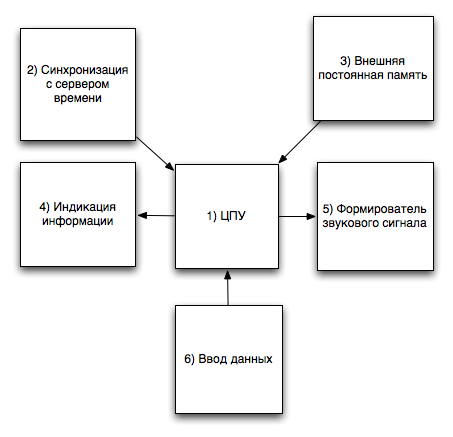
\includegraphics[bb=0 0 453 437, clip, scale=0.8]{funcd.png}}
	\caption{Фнкциональная структура}
	\label{img:funcd}
\end{figure}

\begin{enumerate}
    \item{}ЦПУ --- основной блок отвечает за отсчёт врени и за организацию канала коммуникации
        между блоками воспроизведения мелодии, хранения данных мелодии, и модуля синхронизации времени.
    \item{}Модуль синхронизации времени модуль отвечает за получение информации о текущем веремни
            от удалённого SNTP сервера.
    \item{}Модуль постоянной памяти отвечает за хранение данных, используемых для формирования
        мелодии будильника.
    \item{}Модуль индикации отвечает за отображение текущего времени и наступившего события
        будильника.
    \item{}Модуль формирования аналогово сигнала иcпользуется для формирования сигнала и проигрывания
            мелодии будильника.
    \item{}Модуль ввода данных используется для устновки текущего времени и задания
        времени срабатывания будильника.
\end{enumerate}


\subsection{Описание работы устройства}
\subsubsection{Центральный микроконтроллер}
\begin{par}
Центральное место в схеме занимает микроконтроллер atxmega32a4. Микропрограмма контроллера
должна быть составлена таким образом, что бы прерывание модуля RTC происходило с частотой 2 Гц.
При приходе прерывания микроконтроллер отсчитывает количество $ \frac{1}{2} $ с. прошедших с момента
включения схемы и выводит текущее время на устройство индикации.
\end{par}

\begin{par}
Программа микроконтроллера должна быть написана на языке C++ для компилятора входящего в поставку
AVR-GCC, с учётом всех допущений указанных в разделе <<Язык программирования микроконтроллра>>.
\end{par}

\subsubsection{Устройство индикации}
\begin{par}
В качестве устройства индикации должен использоваться TFT ЖК-дисплей DST2001PH\cite{display} со встроенным
драйвером ili9320 включённым в режиме system i80 16-бит\cite{ili9320}.
Так как количество портов\\*
ввода-вывода на используемом микроконтролере достаточно, введение дополнительных узлов
расширяющих возможности 
ввода-вывода микроконтроллера --- не предусматривается.
\begin{figure}[h]
	\center{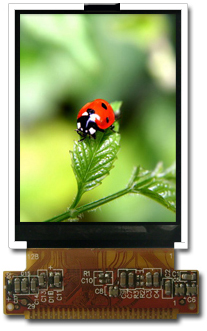
\includegraphics[bb=0 0 150 250, clip, scale=1.0]{ili9320.png}}
	\caption{Внешний вид TFT ЖК-дисплея DST2001PH}
	\label{img:iili9320}
\end{figure}
\end{par}



\begin{par}
В начальный момент работы, устройство должно погасить изображение на ЖК-дисплее и подготовить внутреннюю
память модуля индикации.
\end{par}

\subsubsection{Ввод данных}
\begin{par}
Модуль ввода данных пользователя должен быть выполнен на сенсорном экране ЖК-дисплея,
выполненного по 4-проводной схеме включения резистивного сенсорного экрана. Для
оцифровки значений плучаемых с сенсорного экрана должны использоваться АЦП\cite{avradc} центрального
микроконтроллера.
\end{par}

\begin{par}
В начальный момент работы устройства, после инициализация внутренней памяти ЖК-дисплея, должна быть
произведена процедура калибровки сенсорного экрана, а полученные коэффициенты далее должны быть
использованы для корректировки показаний снятых с сенсорного экрана. Это позволит отказаться
от дополнительной схемы температурной компенсации и статических калибровочных показателей,
и при этом устройство будет выдавать давольно стабильный результат,
так как эксплуатироваться устройство будет в условиях постоянной комнатной температуры,
а собственная рассеиваемая мощьность устройства не должна быть велика на столько, что бы
вносить ощутимую погрешность в показания.
\end{par}


\subsubsection{Звуковое оповещение о наступившем событии}
\begin{par}
Звуковое оповещение о наступившем событии должно быть выполнено на широко распростонённой
микросхеме mc34119, включённой в стандартном режиме (рис. \ref{img:mc34119m}).
\begin{figure}[h]
	\center{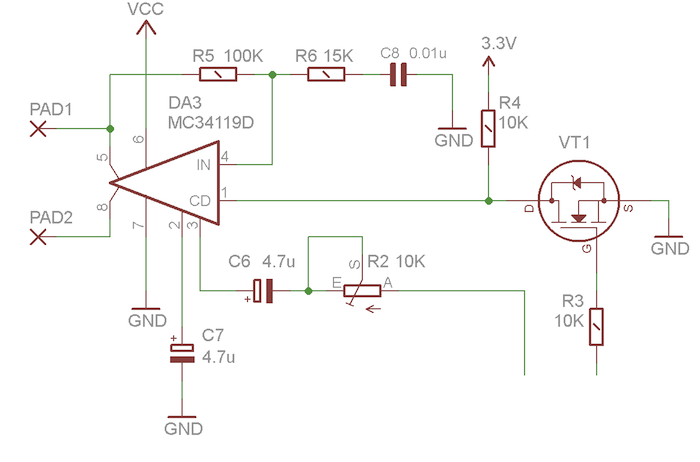
\includegraphics[bb=0 0 200 190, clip, scale=0.8]{mc34119.png}}
	\caption{Схема включения mc34119}
	\label{img:mc34119m}
\end{figure}
\end{par}

\begin{par}
В начальном состоянии на вход Chip Disable микросхемы mc34119 должен подаваться сигнал высокого уровня.
Это переводит микросхему в состояние низкого энергопотребления \cite{mc34119}.
\end{par}

\begin{par}
В момент наступления события будильника на вход Chip Disable микросхемы необходимо подать сигнал 
низкого уровня, выполнить задержку не менее 40 мс., необходимую для перевода микросхемы в
нормальное состояние, и затем подавать на неё вход сигнал с ЦАП центрального микроконтроллера.
Принципиальная схема ЦАП микроконтроллеров AVR семейства XMega приведена на рисунке \ref{img:avrdacp}.
\begin{figure}[h]
	\center{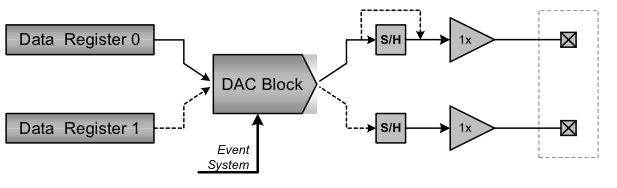
\includegraphics[bb=0 0 300 100, clip, scale=0.8]{avrdac.png}}
	\caption{Принципиальная схема ЦАП микроконтроллеров AVR семейства XMega}
	\label{img:avrdacp}
\end{figure}
\end{par}

\begin{par}
Для воспроизведения музыкального отрывка необходимо использовать нижние 8 бит 12-битного
ЦАП микроконтроллера. Опорное напряжение ЦАП микроконтроллера должно быть равно либо внутреннему
напряжению микроконтроллера 1 В, либо стабилизированному напряжению питания ($AV_{cc}$). Выбор того или иного
опорного напряжения ЦАП обусловливается параметрами динамика и необходимым уровнем громкости.
Для переодического получения данных и их переноса в буфер воспроизведения необходимо использовать
обработик прерывания таймера Timer 1 микроконтроллера. Частота срабатывания таймера выбирается
в соответствии с частотой дискретизации музыкального отрывка.
Механизм программирования ЦАП микроконтроллеров AVR семейства XMega детально описан в документации\cite{avrdac}.
\end{par}


\subsubsection{Устройство хранеия музыкальных отрывков}
\begin{par}
В качестве устройства хранения звуковых отрывков необходимо использовать энергонезависимые карты
памяти MicroSD. Применение этого вида памяти позволит не пребегая к перепрограммированию устройства
вносить музыкальные фрагменты на карту с персонального компьютера, оснащённого модулем
чтения/записи карт MicroSD.
\end{par}

\begin{par}
Для воспроизведения звуковых отрывков центральным микроконтроллером должен быть
организован буфер воспроизведения, таким образом, что бы в случае отсутствия карты MicroSD или
сбоя доступа к ней, в него вносились записанные на этапе программирования данные EEPROM микроконтроллера.
\end{par}

\begin{par}
Для чтения данных карт памяти MicroSD должен использоваться SPI режим работы. Методика программирования
интерфейса SPI микроконтроллеров AVR семейства XMega дана в документации \cite{avrspi}.
\end{par}

\subsubsection{Синхронизация времени}
\begin{par}
В качестве контроллера сетевого интерфейса необходимо использовать микроконтроллер фирмы Micro Chip
enc28j60. Пример включения этого микроконтроллера дан на рисунке \ref{img:ienc28j60}.
\begin{figure}[h]
	\center{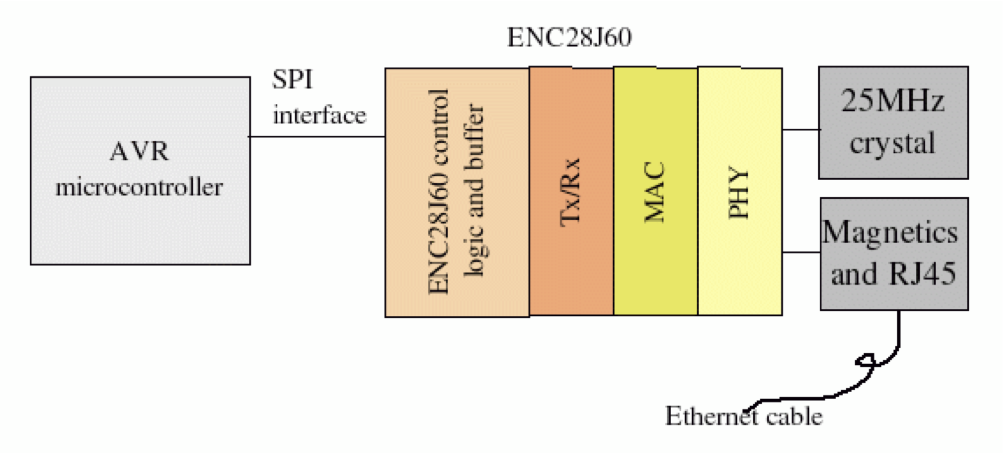
\includegraphics[bb=0 0 500 220, clip, scale=0.6]{enc28j60.png}}
	\caption{Схема включения микроконтроллера enc28j60}
	\label{img:avrdacp}
\end{figure}

Этот микроконтроллер требует использования трансформатора с отношением 1:1 сертефицированного
для сетей 10base-T. По этому для упрощения изделия необходимо использовать готовые RJ45
коннекторы ''Magjack'', которые включают в своей конструкции необходимые трансформаторы и
свето диоды. В случае использования этого метода в схему устройства необходимо будет добавить
только одну индуктивность в 10 мкГн.
\end{par}

\begin{par}
Один раз в 30 минут устройство должно повышать рабочую частоту микроконтроллера до частоты 32 МГц.
И производить попытку синхронизации времени с удалённым SNTP сервисов. По завершению процедуры
синхронизации времени, устройство должно вновь перевести микроконтроллер на рабочую частоту 2 МГц.
\end{par}

\begin{par}
Взаимодействие центрального микроконтроллера и микроконтроллера сетевого интерфейса осуществляется
по протоколу SPI \cite{enc28j60}, расширенному дополнительными сигнальными линиями.
\end{par}


\subsection{Проектирование принципиальной схемы и печатной платы}
\begin{par}
Необходимо разработать принципиальную схему и печатную плату устройства в системе автоматизированного
проектирования Eagle.
\end{par}

\begin{par}
Необходимо разработать схемотическое обозначение и посадочное мето для подключения ЖК-дисплея.
\end{par}

\begin{par}
Необходимо провести DRC проверку выполненой печатной платы на соотвествие параметрам:
\begin{itemize}
    \item{} Количество слоев: до 2;
    \item{} максимальный размер платы (размер рабочего поля): 380х320 мм;
    \item{} минимальная ширина проводника/минимальный зазор: 0,24/0,24 мм;
    \item{} минимальный отступ полигона: 0,24 мм;
    \item{} минимальный диаметр отверстия/минимальная площадка на переходном отверстии: 0,2/0,6 мм;
    \item{} минимальной диаметр монтажного отверстия — 0,6 мм;
    \item{} размер минимальной контактной площадки: для металлизированных отверстий 1,2—1,6 мм — +0,55 мм;
    \item{} минимальная толщина линии шелкографии (маски) — 0,15 мм;
    \item{} минимально допустимое отторжение маски от КП — 0,1 мм, для КП ИМС с шагом 0,5 мм — 50 мкм;
    \item{} минимальная высота шрифта шелкографии — 1,5 мм.
\end{itemize}
\end{par}

\subsection{Разработка SNTP сервиса}
\begin{par}
Необходимо разработать SNTP сервис на языке ErLang. Дополнительных требований к проектированию этого сервиса
не предъявляется, так как основное его назначение --- получение более удобного
инструмента отладки подпрограммы синхронизации времени усройства с удалёнными SNTP сервисами.
При этом делается допущение, что успешный результат испытания по синхронизации свремени с разрабатываемым
сервисом, подтверждает правильность работы как самого сервиса, так и микропрограммы устройства.
\end{par}
\newpage{}
